%% 
%% Authors:  
%% Nils Barrellon (nils.barrellon1@etu.sorbonne-universite.fr)



%%%%%%%%%%%%%%%%%%%%%%%%%%%%%%%%%%%%%%%%%%%%%%%%%%%%%%%%%%%
%% Type et package

\documentclass[a4paper,12pt]{article}
\usepackage[french,english]{babel}
\usepackage{fancyhdr}
\usepackage[utf8]{inputenc}
\usepackage{cmbright}
\usepackage{epsfig}
\usepackage{calc}
\usepackage{url}
\usepackage{boxedminipage}
\usepackage{graphicx}
\usepackage[T1]{fontenc}
\usepackage{hyperref}
\usepackage{csquotes}         % Gère les guillemets
\usepackage[backend=biber,style=numeric]{biblatex} % Pour la bibliographie
\usepackage{float}
\usepackage{listings}
\usepackage{xcolor}
\usepackage{tikz}
\usetikzlibrary{matrix}
\usepackage{enumitem}
\usepackage{amsmath}
\usetikzlibrary{arrows.meta}
\usetikzlibrary{graphs, graphs.standard, quotes}




%%%%%%%%%%%%%%%%%%%%%%%%%%%%%%%%%%%%%%%%%%%%%%%%%%%%%%%%%%%
%%%%%%%%%%%%%%%%%%%%%%%%%%%%%%%%%%%%%%%%%%%%%%%%%%%%%%%%%%%
%% Définitions à personnaliser 

\def\nomEtudA{Nils Barrellon 21401602}

\def\titreProjetLong{RITAL : Chirac ou Mitterrand ? Comm' positif ou négatif ?}

\def\typeDoc{Rapport final}
 
%% - Reglage pour le code inséré

\definecolor{codegray}{gray}{0.95}
\lstset{
inputencoding=utf8,
  literate=
    {é}{{\'e}}1 {è}{{\`e}}1 {ê}{{\^e}}1 {ë}{{\"e}}1
    {É}{{\'E}}1 {È}{{\`E}}1 {Ê}{{\^E}}1
    {à}{{\`a}}1 {â}{{\^a}}1 {ä}{{\"a}}1
    {ù}{{\`u}}1 {û}{{\^u}}1 {ü}{{\"u}}1
    {ô}{{\^o}}1 {ö}{{\"o}}1
    {î}{{\^i}}1 {ï}{{\"i}}1
    {ç}{{\c{c}}}1 {Ç}{{\c{C}}}1,
  language=Python,
  backgroundcolor=\color{codegray},
  basicstyle=\ttfamily\small,
  frame=single,
  breaklines=true,
  keywordstyle=\color{blue},
  commentstyle=\color{gray},
  stringstyle=\color{orange},
  showstringspaces=false ,
  tabsize=3
}



%%%%%%%%%%%%%%%%%%%%%%%%%%%%%%%%%%%%%%%%%%%%%%%%%%%%%%%%%%%
%%%%%%%%%%%%%%%%%%%%%%%%%%%%%%%%%%%%%%%%%%%%%%%%%%%%%%%%%%%
%% Définitions à ne pas modifier
 
%%%%% ||| Mise en page verticale ||| 
\setlength{\voffset}{-1in} % a4:reste 297mm pour les 5 suivants:
\setlength{\topmargin}{15mm}         % avant l'en-tête
\setlength{\headheight}{20mm}        % hauteur de l'en-tête 
\setlength{\headsep}{10mm}            % entre l'en-tête et le corps
\setlength{\textheight}{220mm}       % hauteur du corps
\setlength{\footskip}{12mm}          % pied de page par rapport au corps 

%%%%% --- Mise en page horizontale ---
\setlength{\hoffset}{-1in} % a4:reste 210mm 
\setlength{\oddsidemargin}{15mm}     % entre hoffset et le corps
\setlength{\evensidemargin}{15mm}    % entre hoffset et le corps
\setlength{\marginparwidth}{0mm}     % largeur de la marge
\setlength{\marginparsep}{0mm}       % séparateur corps marge
\setlength{\textwidth}{170mm}        % largeur du corps

\def\annee{2025-26}
\setlength{\parindent}{0cm} 
\renewcommand{\familydefault}{\sfdefault}


%%%%%%%%%%%%%%%%%%%%%%%%%%%%%%%%%%%%%%%%%%%%%%%%%%%%%%%%%%%
%% Début du document

\begin{document}
%\sffamily
\selectlanguage{french}
\setcounter{page}{1} % Réinitialisation des numéros de page



%%%%%%%%%%%%%%%%%%%%%%%%%%%%%%%%%%%%%%%%%%%%%%%%%%%%%%%%%%%
%% Définition des en-têtes et pied de pages
\pagestyle{fancyplain}
\lhead[\fancyplain{}{Master Informatique\\ UE \textbf{RITAL} fév. \annee \\}]
      {\fancyplain{}{Master Informatique\\ UE \textbf{RITAL} \annee}}
\rhead
      {\fancyplain{}{\nomEtudA}}
\lfoot[\fancyplain{}{
\includegraphics[width=3cm]{LOGO_SCIENCES_DEF_CMJN_med.jpg}}]
      {\fancyplain{}{
\includegraphics[width=3cm]{LOGO_SCIENCES_DEF_CMJN_med.jpg}}}
\cfoot[\fancyplain{}{\textbf{\thepage}}]
      {\fancyplain{}{\textbf{\thepage}}}


%%%%%%%%%%%%%%%%%%%%%%%%%%%%%%%%%%%%%%%%%%%%%%%%%%%%%%%%%%%

~

      \begin{center}
        \begin{boxedminipage}{12cm}{
            \begin{center}
              ~\\\LARGE\textbf{\titreProjetLong}\\
              ~\\\large Etudiant: \textbf{\nomEtudA}\\
              ~
            \end{center}
            }
        \end{boxedminipage}
      \end{center}

~

\vspace{2cm}

\begin{center}
\href{https://github.com/nbarrellon/RITAL2026}{Github associé : https://github.com/nbarrellon/RITAL2026}
\end{center}
\vspace{1cm}

\begin{center}
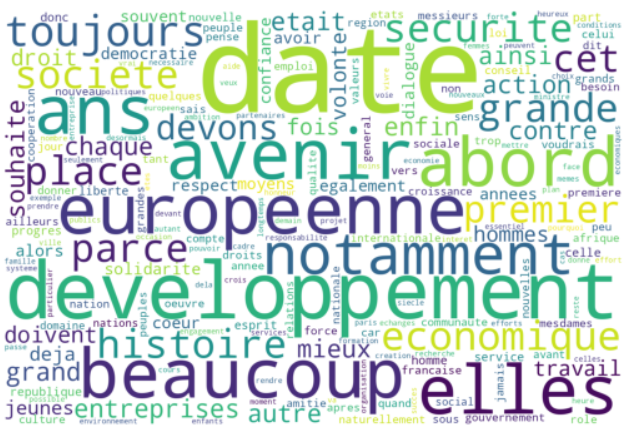
\includegraphics[width=0.8\textwidth]{wordcloud.png} 
\end{center}
        
        


\newpage

\section{Formulation du problème}

\underline{Chirac ou Mitterrand} : on dispose de la transcription d'un débat entre les deux présidents de la République, MM Chirac et Mitterrand. Chaque phrase prononcée par l'un ou l'autre est labellisée. On attribue le label M pour celles proposées par M.Mitterrand que l'on convertit en -1 et le label C (converti en 1) si c'est M.Chirac qui parle. 

Les phrases labellisées de ce débat constitueront donc les données d'entraînement.

L'objectif du projet est de pouvoir attribuer à son auteur une phrase quelconque prononcée dans un autre contexte : on parle de \textbf{diarisation du locuteur}.\\

\underline{Commentaire positif ou négatif} : la dataset est constituée d'une banque de commentaires autour de différents films. L'objectif est de décider si tel ou tel commentaire est un commentaire positif ou négatif : on parle ici d'\textbf{analyse de sentiment}. 

\section{Etude du problème de diarisation du locuteur}

\subsection{Bag of words}

J'ai créé différents bag of words (\textit{bog}) pour les documents afin d'en tester la pertinence.
%------------------------------------------------------------------------------------------
\subsubsection{Pré-processing}

J'effectue en amont de la construction du \textit{bog} un nettoyage du texte. Les options retenues sont :
\begin{itemize}
\item suppression de la ponctuation ;
\item suppression des chiffres ;
\item mise en minuscule ;

\end{itemize} 

Ce nettoyage est opéré par ma fonction personnalisée de pré-processing suivante :

\begin{lstlisting}
import codecs
import re 
import string
from unidecode import unidecode

def preprocessPerso(text): 
    #suppression de la ponctuation
    punc = string.punctuation
    punc += '\n\r\t'
    text = text.translate(str.maketrans(punc, ' '*len(punc)))
    #suppression des chiffres
    text = re.sub(r"[0-9]","",text)
    #suppression des accents
    text = unidecode(text)
    #mise en minuscule
    return text.lower()
\end{lstlisting}
%------------------------------------------------------------------------------------------
\subsubsection{Stopwords}
Je supprime les mots blancs avant construction du \textit{bog}. La liste des stopwords est obtenue par concaténation des stopwords français donnés par la bibliothèque \texttt{nltk} auxquels j'ajoute une liste personnelle, établie à partir de la liste des mots les plus présents et non-discriminants.

\begin{lstlisting}
# Mots blancs + mots les plus fréquents

nltk.download('stopwords')
from nltk.corpus import stopwords
final_stopwords_list = stopwords.words('french')
#mots les plus fréquents donc non-discriminants
final_stopwords_list += ['ai','au','aujourd','aussi','autres','aux','avec','avez' ,'avons',
 'bien', 'ce' ,'cela', 'ces', 'cette' ,'ceux', 'chacun' ,'comme', 'dans' ,'date'
 'de', 'depuis', 'des' ,'deux' ,'dire' ,'doit' ,'dont' ,'du'
 'elle' ,'en' ,'encore', 'ensemble', 'entre', 'est' ,'et', 'etat', 'ete' ,'etre',
 'europe' ,'faire' ,'fait' ,'faut', 'francais' ,'france', 'hui' ,'ici', 'il' ,'ils',
 'je' ,'la', 'le' ,'les', 'leur' ,'leurs', 'mais', 'meme' ,'monde', 'monsieur' ,'ne',
 'nom', 'nos', 'notre', 'nous', 'on', 'ont' ,'ou', 'paix', 'par', 'pas', 'pays',
 'peut' ,'plus' ,'politique' ,'pour', 'president' ,'qu', 'que' ,'qui', 'sa', 'sans',
 'se' ,'ses' ,'si' ,'son' ,'sont', 'sur', 'temps', 'tous', 'tout', 'toute' ,'toutes',
 'tres', 'un' ,'une' ,'union', 'vie', 'vos' ,'votre', 'vous']
\end{lstlisting}

Cette liste a été obtenue à l'aide du script ci-dessous :
\begin{lstlisting}
from sklearn.feature_extraction.text import TfidfVectorizer

use_idf=True
smooth_idf=True
sublinear_tf=False

vectorizer = TfidfVectorizer(preprocessor=preprocessPerso,use_idf= use_idf, smooth_idf=smooth_idf, sublinear_tf=sublinear_tf,max_features=100)
BOW1 = vectorizer.fit_transform(alltxts)
vocabulaire = vectorizer.get_feature_names_out()
\end{lstlisting} 
%------------------------------------------------------------------------------------------
\subsubsection{Premier bog}

Bag of words simple. Taille du vocabulaire =  26894
\begin{lstlisting}
vectorizer1 = CountVectorizer(stop_words=final_stopwords_list,analyzer="word", preprocessor=preprocessPerso)
BOW1 = vectorizer1.fit_transform(alltxts)
\end{lstlisting}


\begin{center}
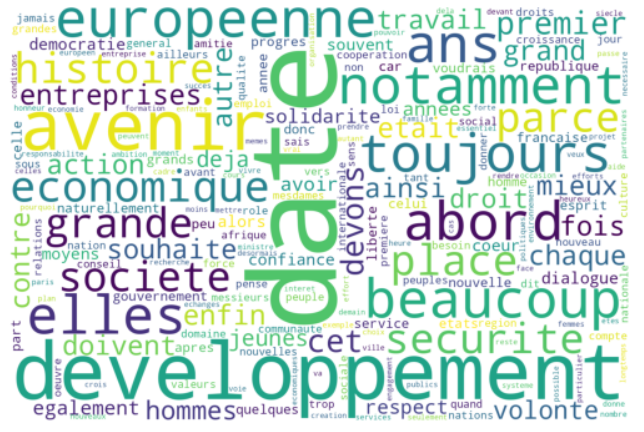
\includegraphics[scale=0.5]{bow1.png}
\end{center}
%------------------------------------------------------------------------------------------
\subsubsection{Deuxième bog}
Utilisation de TF-IDF. Nombre de mots du vocabulaire: 2000
\begin{lstlisting}
use_idf=True
smooth_idf=True
sublinear_tf=False

vectorizer2 = TfidfVectorizer(use_idf= use_idf, smooth_idf=smooth_idf,\
sublinear_tf=sublinear_tf,                      preprocessor=preprocessPerso,stop_words=final_stopwords_list,max_features=2000)
BOW2 = vectorizer2.fit_transform(alltxts)

\end{lstlisting}


\begin{center}
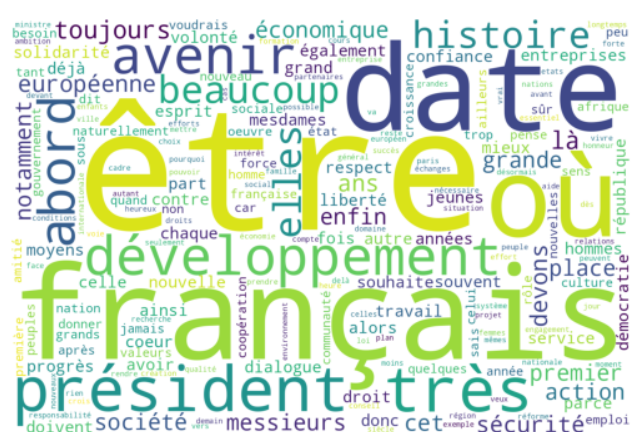
\includegraphics[scale=0.5]{bow2.png}
\end{center}
%------------------------------------------------------------------------------------------
\subsubsection{Troisième bog}
Utilisation des bigrammes. Taille du vocabulaire =  328573
\begin{lstlisting}
ngram_range = (1,2)
vectorizer3 = CountVectorizer(ngram_range=ngram_range,analyzer='word',stop_words=final_stopwords_list,preprocessor=preprocessPerso)
BOW3 = vectorizer3.fit_transform(alltxts)

\end{lstlisting}


\begin{center}
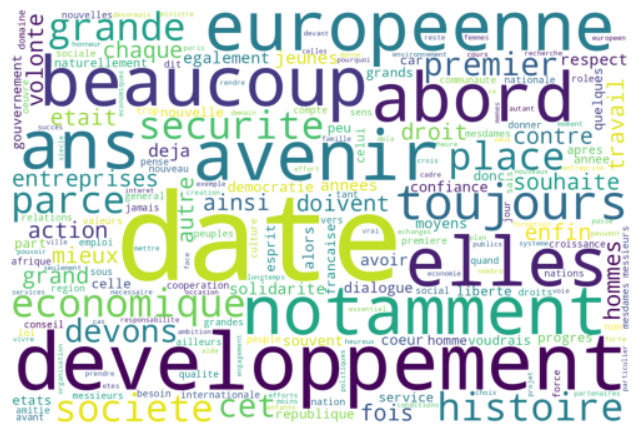
\includegraphics[scale=0.5]{bow3.png}
\end{center}
%------------------------------------------------------------------------------------------
\subsubsection{Quatrième bog}
On utilise la racinisation avant construction du \textit{bog}. 
\begin{lstlisting}
nlp = spacy.load("fr_core_news_sm", disable=["parser", "ner"]) 

def lemmatisation(text, stopwords):
    text = preprocessPerso(text)
    doc = nlp(text.lower())
    # Lemmatiser uniquement les mots qui ne sont pas des stopwords
    lemmatized = [token.lemma_ for token in doc if token.text not in stopwords]
    text = " ".join(lemmatized).strip()
    #on supprime les espaces surnuméraires créés par la racinisation
    text = re.sub(r'\s+', ' ', text)
    return text

# Pré-traiter tous les textes
alltxts_lemmatise = []
for text in alltxts:
    alltxts_lemmatise.append(lemmatisation(text, final_stopwords_list))
    
\end{lstlisting}

Le résultat est très probant comme le montre l'exemple ci-dessous (1$^{ère}$ phrase du débat avant et après racinisation) :

\begin{verbatim}
C'est toujours très émouvant de venir en Afrique car c'est probablement 
l'une des rares terres du monde où l'on ait conservé cette convivialité, 
cette amitié, ce respect de l'autre qui s'expriment avec chaleur, avec spontanéité 
et qui réchauffent le coeur de ceux qui arrivent et de ceux qui reçoivent.

-------------------------------
être toujours tre emouver venir afrique car être probablement rare terre avoir
conserve convivialite amitie respect autre exprimer chaleur spontaneite rechauffer 
coeur celui arriver celui recoiver
\end{verbatim}
Taille du vocabulaire =  19049\\

Je note que, sans surprise, les auxiliaires \textbf{être} et \textbf{avoir} arrivent en tête des mots les plus fréquents. Je décide donc de les ajouter aux mots blancs.

\underline{A noter:} ce processus de racinisation est très long et j'ai donc sauvegardé le vocabulaire obtenu pour ne pas avoir à le recalculer à chaque fois. 

\begin{lstlisting}
with open("corpus_nettoye_lemmatise.txt","w",encoding="utf-8") as f:
    for i in range(len(alltxts_lemmatise)):
        f.write(alltxts_lemmatise[i])
        f.write("\n")
\end{lstlisting}

\begin{center}
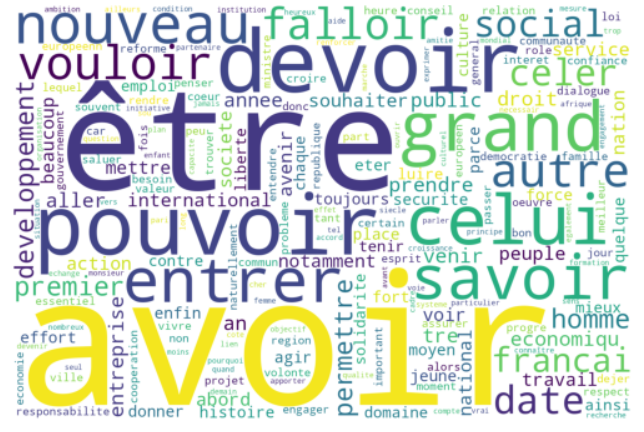
\includegraphics[scale=0.5]{bow4.png}
\end{center}
%------------------------------------------------------------------------------------------
\subsubsection{Cinquième bog}
Je conjugue bigrammes et racinisation. Taille du vocabulaire =  345610
\begin{lstlisting}
ngram_range = (1,2) 
final_stopwords_list += ['avoir',"être"]
vectorizer5 = CountVectorizer(ngram_range=ngram_range,analyzer='word',\
stop_words=final_stopwords_list,preprocessor=preprocessPerso) 
BOW5 = vectorizer5.fit_transform(alltxts_lemmatise)
\end{lstlisting}
\begin{center}
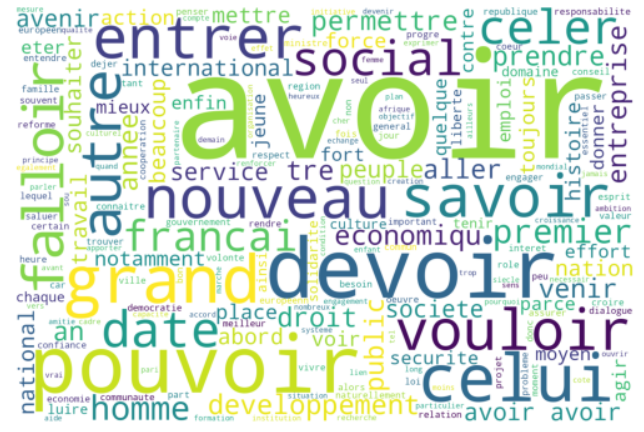
\includegraphics[scale=0.5]{bow5.png}
\end{center}

Je note que les mots les plus fréquents sont des monogrammes.
%------------------------------------------------------------------------------------------
\subsubsection{Sixième bog}
Je construis un bog binaire. Taille du vocabulaire =  10000
\begin{lstlisting}
min_df=5
max_df=0.5
max_features=10000
vectorizer6 = CountVectorizer(max_df=max_df,min_df=min_df,max_features=max_features,\
binary=True,stop_words=final_stopwords_list) 
BOW6 = vectorizer6.fit_transform(alltxts)
\end{lstlisting}
\begin{center}
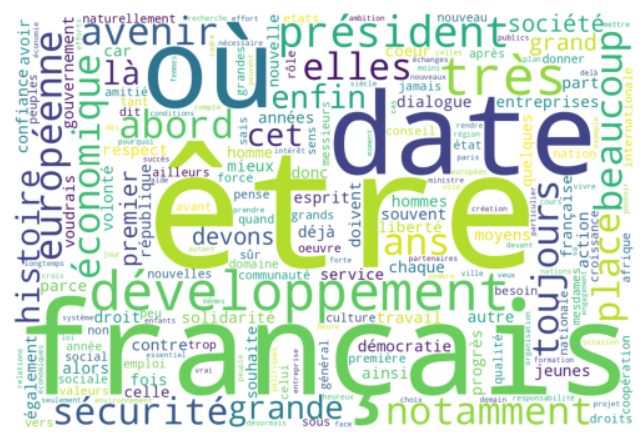
\includegraphics[scale=0.5]{bow6.png}
\end{center}

%------------------------------------------------------------------------------------------
\subsubsection{Septième bog}
J'applique une racinisation avant un TF-IDF. Taille du vocabulaire = 4000
\begin{lstlisting}
use_idf=True
smooth_idf=True
sublinear_tf=False
vectorizer7 = TfidfVectorizer(use_idf= use_idf, smooth_idf=smooth_idf, sublinear_tf=sublinear_tf,\
                            stop_words=final_stopwords_list,max_features=4000)
BOW7 = vectorizer7.fit_transform(alltxts_lemmatise)
\end{lstlisting}
%------------------------------------------------------------------------------------------
\subsubsection{Huitième bog}
J'applique une racinisation avant un TF-IDF sur des bigrammes. Taille du vocabulaire = 4000
\begin{lstlisting}
use_idf=True
smooth_idf=True
sublinear_tf=False
vectorizer8 = TfidfVectorizer(use_idf= use_idf, smooth_idf=smooth_idf, sublinear_tf=sublinear_tf,\
                            stop_words=final_stopwords_list,max_features=4000)
BOW8 = vectorizer8.fit_transform(alltxts_lemmatise)
\end{lstlisting}

\subsubsection{Neuvième bog}
Je me suis aperçu, en séparant les données par locuteur en 2 corpus distincts, que M.Chirac a beaucoup plus parlé que M.Mitterrand lors de ce débat. 

\begin{lstlisting}
corpus1 = [alltxts[i] for i in range(len(alltxts)) if alllabs[i]==1] #Chirac
corpus2 = [alltxts[i] for i in range(len(alltxts)) if alllabs[i]==-1] #Mitterand

#Taille des corpus
print("------------------Taille des corpus-----------------------")
print("Chirac:",len(corpus1))
print("Mitterrand",len(corpus2))
\end{lstlisting}

\begin{verbatim}
------------------Taille des corpus-----------------------
Chirac: 49890
Mitterrand 7523
\end{verbatim}

Ceci a une influence considérable sur l'entrainement et les prédictions des différents modéles. La métrique de la précision, très bonne quelque soit le \textit{bog} utilisé, n'est plus pertinente. \\ 

Il m'a donc semblé pertinent de ré-équilibrer les données. J'ai donc créé un neuvième \textit{bog} en ramenant le nombre d'interventions de M.Chirac à un nombre égal à celui de M.Mitterrand. 

\begin{lstlisting}
corpus1 = [(alltxts_lemm[i],alllabs[i]) for i in range(len(alltxts)) if alllabs[i]==1] #Chirac
corpus2 = [(alltxts_lemm[i],alllabs[i]) for i in range(len(alltxts)) if alllabs[i]==-1] #Mitterand

corpus = corpus2+corpus1[:len(corpus1)//6]
new_alltxts = [c[0] for c in corpus]
new_labels = [[c[1] for c in corpus]]

ngram_range = (1,2) # unigrams and bigrams

use_idf=True
smooth_idf=True
sublinear_tf=False

vectorizer9 = TfidfVectorizer(ngram_range=ngram_range,analyzer="word",use_idf= use_idf, smooth_idf=smooth_idf, sublinear_tf=sublinear_tf,\
                            stop_words=final_stopwords_list,max_features=5000)
BOW9 = vectorizer9.fit_transform(new_alltxts)
\end{lstlisting}

Taille du vocabulaire = 5000

\begin{center}
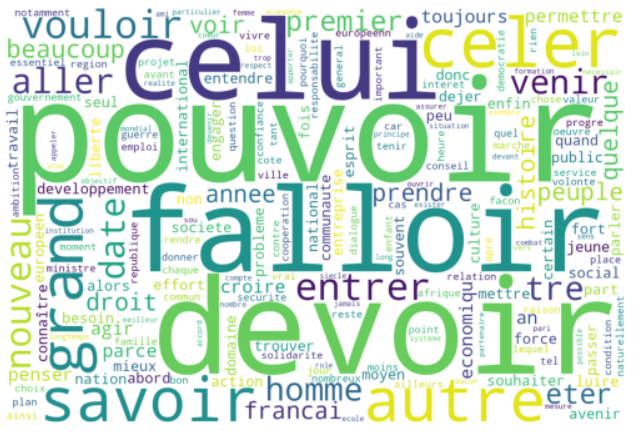
\includegraphics[scale=0.5]{bow9.png}
\end{center}
%------------------------------------------------------------------------------------------
\section{Classificateurs}

J'applique trois méthodes de classification sur mes différents \textit{bog} :
\begin{itemize}
\item Naïve Bayes
\item Regression logique
\item SVD
\end{itemize}

La méthode \textbf{Naïve Bayes} applique le théorème de Bayes en supposant que les mots sont indépendants entre eux (d'où le "naïf"). Pour un texte, il calcule la probabilité que chaque mot appartienne à chaque classe, puis multiplie ces probabilités pour classer le document. \\


La \textbf{régression logistique} modélise la probabilité d'appartenir à une classe via une fonction sigmoïde appliquée à une combinaison linéaire des mots. C'est un modèle linéaire qui une frontière de décision droite entre les classes. \\

La méthode \textbf{SVM pour Support Vector Machine} cherche l'hyperplan qui sépare les classes avec la marge maximale entre les points les plus proches de chaque classe (les vecteurs de support). Grâce à l'astuce du kernel, il peut projeter les données dans un espace de dimension supérieure pour séparer des classes non linéairement séparables. 

\section{Métriques}

J'ai testé les 3 méthodes de classification sur chacun des \textit{bog} et mesuré 3 métriques différentes sur les données test : la précision, le rappel et le f1-score. La figure montre de plus le temps d'exécution des 3 modèles pour chaque \textit{bog}.
\begin{center}
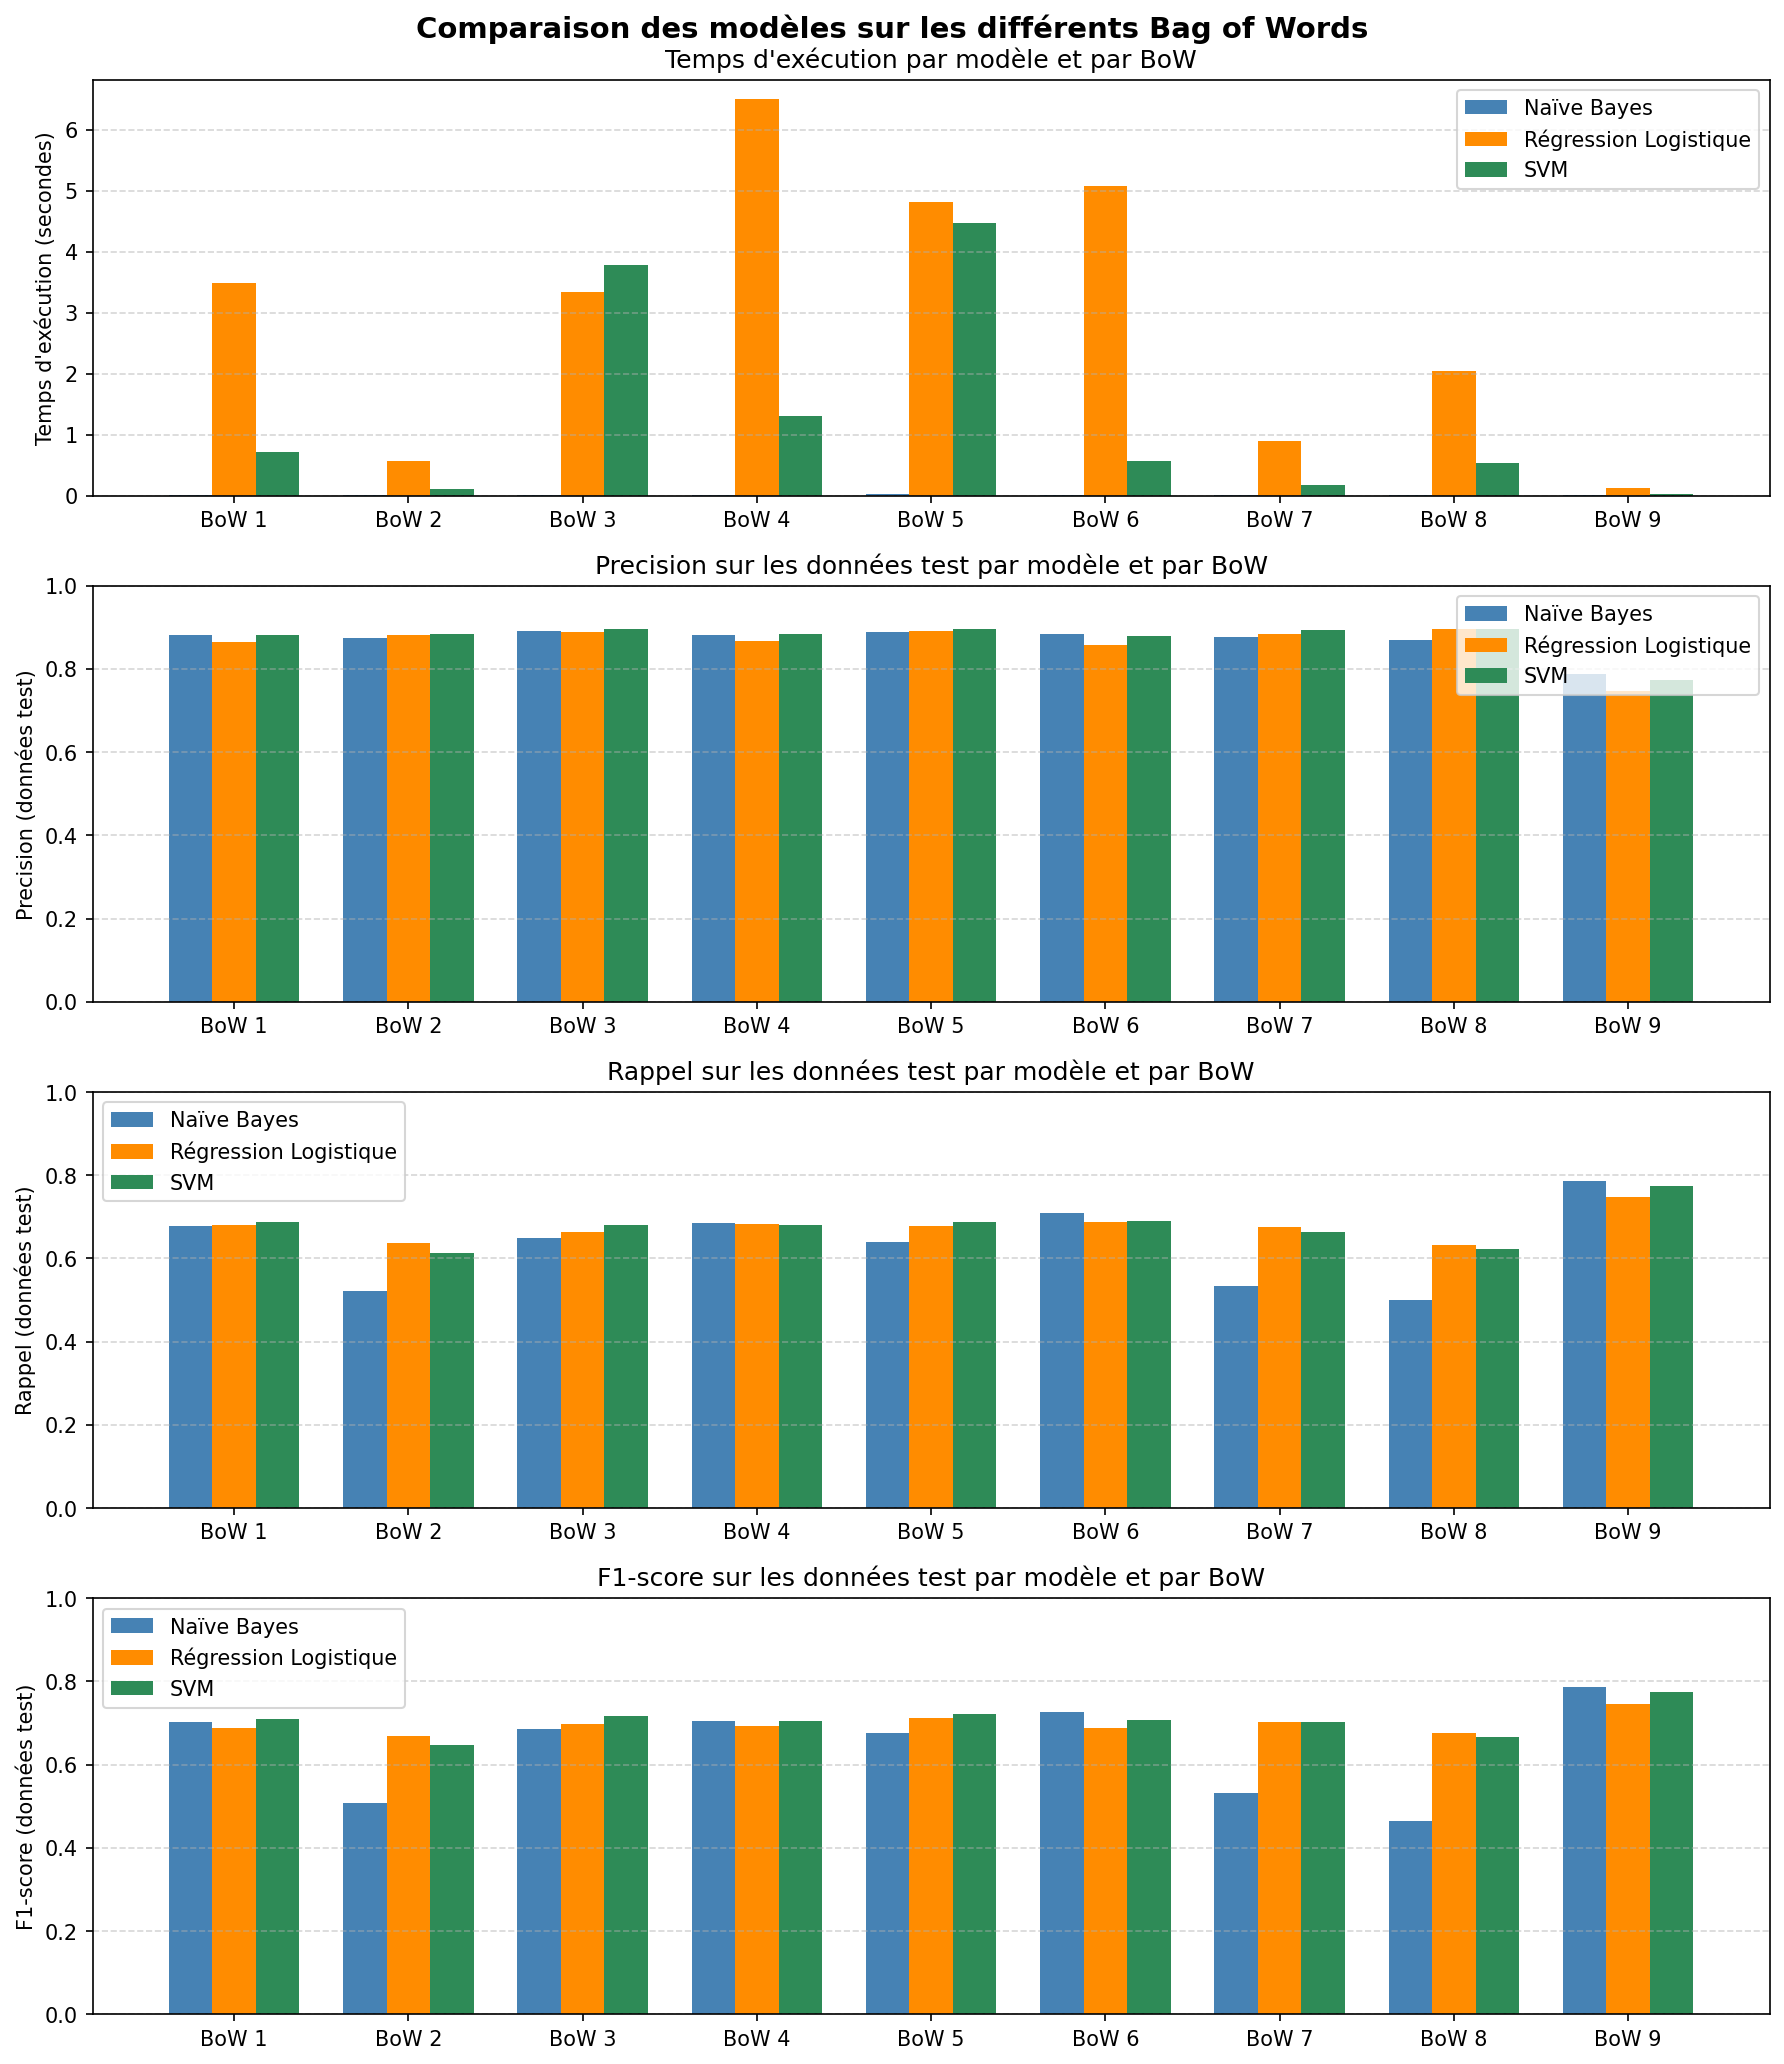
\includegraphics[scale=0.5]{bow_comparaison.png}
\end{center}
 
Le ré-équilibrage des données semble mener à un résultat de meilleure qualité. J'ai donc testé ce \textit{bog} pour ma première soumission de données sur la plateforme.

Voici le script que j'ai utilisé pour générer mon fichier de résultats :

\begin{lstlisting}
#Choix du bog
vectorizer = vectorizer9 

#Application du BOG sur les données à tester
test_nouvelles_phrases = vectorizer.transform(nouvelles_phrases)

X_train = BOW9
y_train = new_labels

#Choix du modèle
model = LogisticRegression(random_state=0, solver='liblinear', max_iter=10
00, tol=1e-8, C=100.0)

# Entrainement du modèle
model.fit(X_train, y_train)


probabilites = model.predict_proba(test_nouvelles_phrases)[:, 1]  # Probabilité classe "Chirac"

# Créer un DataFrame avec les probabilités
df = pd.DataFrame({
    "phrase": nouvelles_phrases,
    "probabilite_chirac": 1-probabilites #car on veut la proba pour Mitterand
})

# Écrire dans un fichier CSV
df.to_csv("probabilites_chirac.csv", index=False, header=False,columns=["probabilite_chirac"])
\end{lstlisting}

Cette première soumission m'a rendu les métriques suivantes :
\begin{itemize}
\item f1 =35.052
\item auc = 70.976
\item ap = 29.524
\end{itemize}

Ces résultats m'ont énormément surpris puisque très différents de ceux obtenus sur les données test. J'ai donc cru que je m'étais trompé de probabilité et ai soumis un nouveau fichier csv contenant \texttt{1-proba}. Les résultats étaient pires. Comment expliquer ces mauvais scores ?

J'ai dans l'idée que la normalisation était inadaptée : la racinisation pourrait bien avoir supprimé des informations utiles. J'ai donc soumis les données obtenues avec le premier \textit{bog}.

Cette deuxième soumission m'a rendu les métriques suivantes :
\begin{itemize}
\item f1 =15.463
\item auc = 29.817
\item ap = 9.285
\end{itemize}

Résultats catastrophiques et incompréhensibles. Une nouvelle fois, j'ai pensé avoir inversé les probabilités mais, après avoir soumis les probabilités inversées les résultats n'étaient pas meilleurs.

Je suis donc revenu aux "basiques" pour ma cinquième soumission. J'ai utilisé un \textit{bog} TF-IDF, avec utilisation des stopwords fournis par la bibliothèque \texttt{nltk} avec mon nettoyage en amont personnel.

\begin{lstlisting}
from nltk.corpus import stopwords
final_stopwords_list = stopwords.words('french')
use_idf=True
smooth_idf=True
sublinear_tf=False

vectorizer10 = TfidfVectorizer(ngram_range=(1,2),analyzer="word",use_idf= use_idf, smooth_idf=smooth_idf, sublinear_tf=sublinear_tf,\
                            stop_words=final_stopwords_list,preprocessor=preprocessPerso)
BOW10 = vectorizer10.fit_transform(alltxts)
\end{lstlisting}

Cette cinquième soumission m'a rendu les métriques suivantes :
\begin{itemize}
\item f1 =56.392
\item auc = 87.603
\item ap = 63.694
\end{itemize}

Résultats meilleurs mais toujours pas satisfaisants. Mon nombre d'essais se rabougrissant comme peau de chagrin, j'ai procédé à une analyse plus poussée en amont de ma prochaine soumission. Notamment en établissant la matrice de confusion de mes prédictions obtenues avec mon dernier \textit{bog}.


\begin{lstlisting}
[X_train, X_test, y_train, y_test]  = train_test_split(BOW10, alllabs, test_size=0.2, shuffle=True)


# Entrainement du modèle
model.fit(X_train, y_train)
y_pred = model.predict(X_test)

#Convertir les labels en 'N' (négatif) ou 'P' (positif)
y_pred_labels = ['M' if lbl <0.5 else 'C' for lbl in y_pred]
y_test_labels = ['M' if lbl==-1 else 'C' for lbl in y_test]
# Matrice de confusion
cm = confusion_matrix(y_test_labels, y_pred_labels)
disp = ConfusionMatrixDisplay(confusion_matrix=cm, display_labels=["Chirac","Mitterrand"])
disp.plot(cmap=plt.cm.Blues)
plt.title("Matrice de confusion")
plt.show()

\end{lstlisting}

J'ai obtenu un résultat surprenant :
\begin{center}
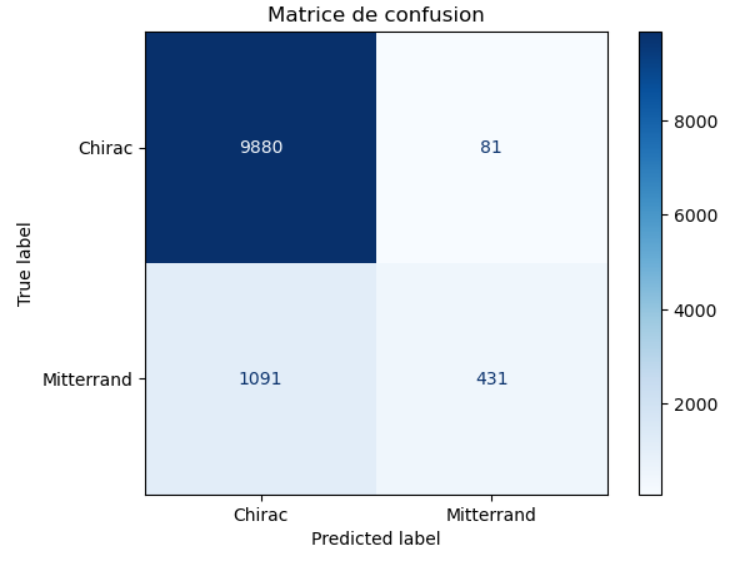
\includegraphics[scale=0.4]{matrice_conf1.png}
\end{center}

Le locuteur Chirac est très bien discriminé. En revanche, l'erreur est la norme pour le locuteur Mitterrand. Ceci allait dans le sens de mes premières observations : M.Chirac a beaucoup plus parlé que M.Mitterrand et le modèle est biaisé.
Ce qui ressort sur la matrice de confusion, réalisé après ré-équilibrage des données brutes.
\begin{center}
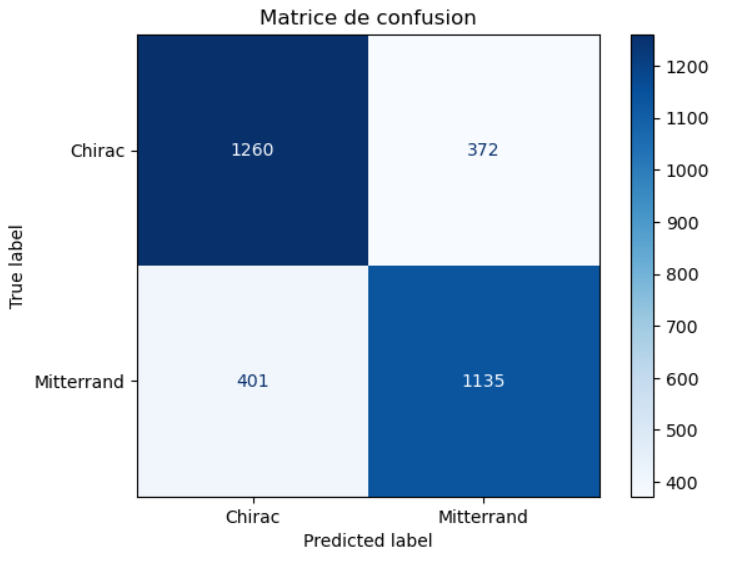
\includegraphics[scale=0.4]{matrice_conf2.png}
\end{center}

J'ai noté une amélioration si je ne restreins pas la taille du vocabulaire...

\begin{center}
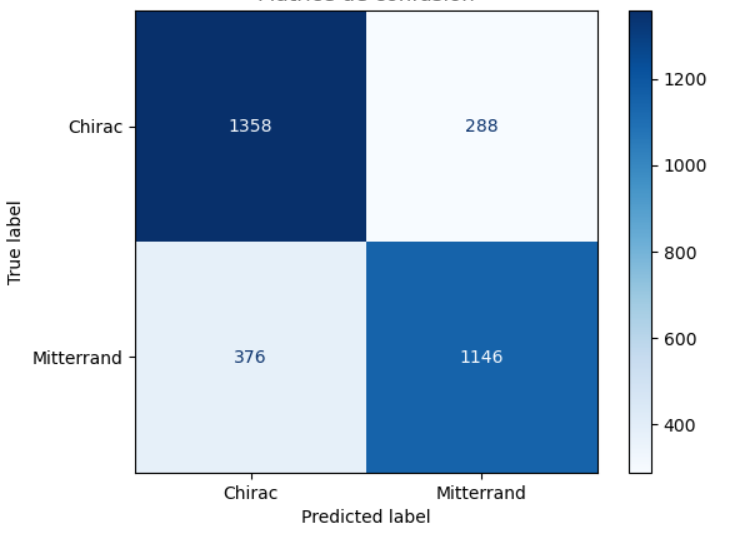
\includegraphics[scale=0.4]{matrice_conf3.png}
\end{center}

Enfin, j'ai renouvelé l'opération de lemmatisation sur les données ré-équilibrées. La matrice de confusion est légèrement meilleure.

\begin{center}
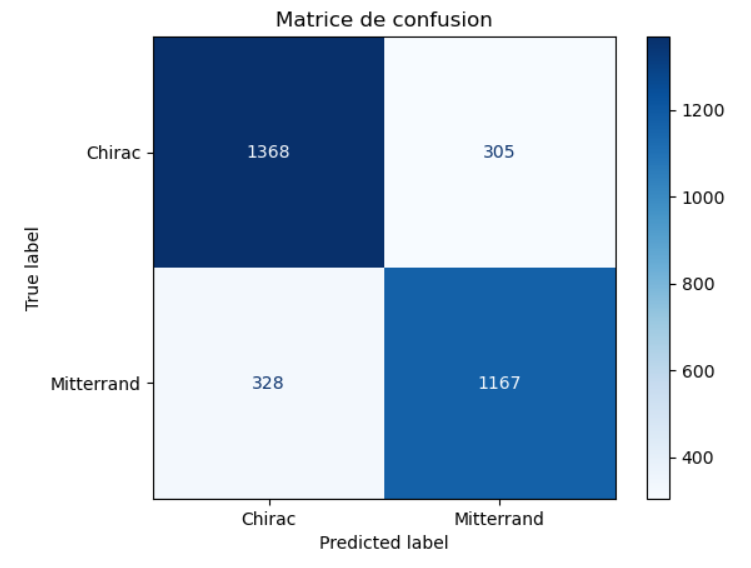
\includegraphics[scale=0.4]{matrice_conf4.png}
\end{center}

Mes deux dernières soumissions me renvoient les métriques suivantes (et donc définitives) :
\begin{itemize}	
\item f1 =79.030
\item auc = 96.970
\item ap = 88.548
\end{itemize}

\subsection*{5 Discussion sur les résultats obtenus et la méthode utilisée}

Il me semble que la méthode utilisant des \textit{bog} atteint ici ses limites.L'empirisme étant de mise, un nombre de soumissions beaucoup plus importants aurait été intéressant. A fortiori car les tests menés sur les données dont nous disposions renvoyaient des résultats assez divergents de ceux des données test (ce que je ne m'explique pas...). Le ré-équilibrage des données a permis toutefois d'obtenir des résultats un peu plus corrects.\\

Je pense aussi, pour avoir essayé, que nous aurions pu jouer sur le seuil de détection. Fixé ici à 0.5, j'ai obtenu des résultats légèrement meilleurs en abaissant ce seuil. \\

Enfin, j'ai eu du mal à saisir les répercussions du travail sur le vocabulaire. Ce qui paraissait évident (comme la suppression des mots blancs ou la racinisation) n'a pas donné les résultats escomptés.

\section{Etude du problème de l'analyse de sentiments}

Ma démarche a été similaire au problème précédent. Création de \textit{bog}. J'ai soumis les résultats obtenues avec les \textit{bog} suivants -- tous ont été construits sans les stopwords anglais :
\begin{itemize}
\item 2-grammes, racinisation et modele SVC;
\item TF-IDF et 5000 mots de vocabulaire (modèle régression logique);
\item BOG simple avec 8000 mots de vocabulaire (modèle régression logique) ;
\item TF-IDF et N-grammes (soumissions n°4 et n°6) (modèle régression logique);
\item BOG binaire (modèle régression logique).
\end{itemize}

Les métriques obtenues ont été sensiblement identiques, au delà de 80\%. Les meilleurs résultats ont été obtenues avec ma première soumission ce qui me semble tout à fait logique. Je pense que la racinisation (stemming) a très bien fonctionné avec la langue anglaise et plus particulièrement avec des commentaires de films qui ne sont généralement pas des parangons de littérature.
\end{document}
